% Background and Significance
% No page limit
\chapter{The lateralization of structure and function in aging: A combined fMRI and DTI study}
\label{chap_lat}

This chapter presents work submitted to the 13th International Conference on Medical Image Computing and Computer Assisted Intervention 2010 Workshop on Computational Diffusion MRI, Beijing, China. Measures from event-related functional MRI, diffusion tensor imaging tractography and cognitive performance in a language-based task were used to test the hypothesis that lateralization of function and structure changes with age and plays a role in regulating cognitive performance.  Functional activation was examined in three functionally activated regions and their opposite hemisphere homologues in healthy young adults and healthy seniors. The health seniors were divided into two groups, one that was cognitively matched with the young adults, and one that performed more poorly on a working memory task. The functional regions were used to identify the white matter fiber tracts that provide the biological connectivity between the activated regions and structural connectivity was measured by averaging fractional anisotropy (FA) over a geometric fiber bundle model that projects local white matter properties onto a centerline. Young adults had symmetric activation patterns. Seniors were found to have higher activation in the right posterior temporal cortex and this activation was higher for higher performing seniors than lower performing seniors. FA in the right hemisphere arcuate fasciculus was found to have higher FA in seniors, but lower FA was found in the right hemisphere short frontal fibers and the posterolateral temporal inter-hemispheric connections of seniors. Higher performing seniors also lower FA in the inferior frontal inter-hemispheric connections compared to lower performing seniors. Right hemisphere compensatory activation in older adults may be due in part to age-related changes in white matter connectivity.


\section{Introduction}
\label{sec:intro}
Lateralization, the asymmetric distribution of cognitive resources between hemispheres, is a distinctive feature of the human brain. The first evidence for functional lateralization was provided by Paul Broca's (1824 - 1880) post-mortem examinations of subjects with language deficits which revealed that the left hemisphere subserves language processing. More detailed examinations of lateralization were conducted by Roger Sperry~\cite{Sperry1974} who conducted a series of experiments testing functional lateralization in subjects whose corpus callosa had been surgically severed in order to prevent epileptic seizures. These experiments demonstrated that when words were presented to the left visual field (i.e. right hemisphere), the subjects did not report seeing anything, but when the words were presented to the right visual field, the subjects were able to correctly report the word. More recently, functional magnetic resonance imaging (fMRI) has provided further evidence confirming that language processing is handled in the left hemisphere~\cite{Frost1999,Bookheimer2002}. Addtionally, diffusion tensor imaging (DTI) tractography has been used to identify hemispheric asymmetries in the white matter tracts that provide the anatomical connections between the cortical regions associated with the language network~\cite{Catani2008,Glasser2008}.
 
Studies of the aging brain have suggested that older adults recruit right hemisphere resources for language processing, however the basis for the compensatory process is not known~\cite{Cabeza2002}. A number of hypotheses have been proposed to explain the changes in functional lateralization that accompany aging. The \emph{compensation view} posits that increased right hemispheric activity is an attempt to counteract age-related neurocognitive decline~\cite{Cabeza1997} whereas the \emph{dedifferentiation view} posits that these increases are are the result of a response to increased difficulty in the recruiting of specialized neural mechanisms~\cite{Li1999}. The \emph{psychogenic view} posits that these changes reflect the implementation of novel cognitive strategies that are not used (and not needed) by younger adults except for very difficult tasks~\cite{Light1991}. This contrasts with the \emph{neurogenic view} which posits that the asymmetry reductions a the result of age-related changes to neuronal architecture. A global reorganization of functional specialization is posited by the \emph{network view} while the \emph{regional view} posits that the asymmetry changes are independent of functional specialization. The \emph{resources view} posits that cognitive processes are fueled by limited resources and that decreased lateralization results from age-related capacity declines in left-hemispheric neural units~\cite{Craik1983}. An age-related decline is processing speed is assumed by the \emph{speed view} which posits that increased recruitment of neurons results in increased processing speed. Finally, the \emph{inhibition view} posits that age-related declines in inhibition result in reduced lateralization resulting in decreased cognitive performance due to greater influence of task-unrelated information~\cite{Hasher1988}. Many of these views are not mutually exclusive, suggesting that the true origin for reduced functional lateralization may be some combination of the above. The evaluation of these views is complicated by a lack of information regarding: the relationship of lateralization and cognitive performance with aging, incidence and age-of onset of decreased lateralization, and gender differences.

To gain further insight into the nature of lateralization changes with aging it is necessary to not only examine functional activity in the brain, but also the structural properties in the biological network that provides the connections that allow inter-hemispheric communication. These inter-hemispheric, or commisural, connections are provide by the corpus callosum, the largest neural pathway in the human brain, incorporating between 200 million and 800 million axons~\cite{Banich1995}. The corpus callosum consists primarily of homotopic connections that connect homolous cortical regions in each hemisphere~\cite{Hellige1993}, but evidence has been found for a small number of heterotopic connections~\cite{Wahl2009}. Studies of the corpus callosum often treat it is a single entity, but previous studies have revealed that different components of the corpus callosum transfer different types of information suggesting that the corpus callosum may be more accurately depicted as a collection of independent pathways~\cite{Banich1995}. The functional role of the corpus callosum is still an open issue with evidence for both inhibitory and excitatory roles~\cite{Yazgan1995}. The balance between inhibition and excitation may be regulated by a balance between the two fiber types that make up the corpus callosum, large diameter fibers that connect sensory-motor areas and small diameter fibers that connect association areas~\cite{Yazgan1995}. The smaller diameter axons are more prevalent and are believed to responsible for individual differences in callosal size~\cite{Bloom2005}. 

In this study, functional subnetworks in the brain were examined using MRI to measure both structure and function during a language processing task. A healthy young adult population was compared to healthy seniors. The seniors were grouped into higher performing and lower performing groups so that functional and structural differences could be examined. Functional regions identified in a previous study~\cite{Gunawardena2009} were used to examine region-averaged activation values. The functional regions were then used to identify the white matter fiber tracts that provide the communication channels between the functional regions. Atlas-based DTI tractography was used to create geometric models of fiber bundles. Deterministic tractography was used to identify the well defined association fibers that connect the functional regions of interest while a shortest-path tractography method is used to identify the inter-hemispheric connections. Structure was quantified with arc-length parameterizations of fractional anisotropy (FA)~\cite{Jones2005,Corouge2006,Maddah2008d,ODonnell2009}. These structural and functional metrics were used to identify possible differences between the young adult and senior populations as well as within the high and low performing senior groups.

\section{Methods}
\label{sec:methods}
Functionally activated regions were defined using fMRI and used to examine functional activation levels in these regions as well as in homologous regions in the opposite hemisphere. The activated regions were used along with diffusion tensor MRI tractography to identify the white matter pathways that provide the biological connectivity of the network. Tract-averaged FA was measured in each fiber tract using a centerline-based method to identify structural differences related to aging. Diffusion tensor images, T1 images and fMRI were acquired for a set of ten young adults and 13 seniors. A working memory test was used to group the seniors into two sets, one that was cognitively matched with the young adults (n=7), and one that performed more poorly on the test (n=6). These groupings are used to examine the relationship between structure and function and their relationship to cognitive performance and aging. 

\subsection{Analyses of fMRI}
A previous study investigated the neural mechanisms that support the resolution of grammatically complex sentences~\cite{Gunawardena2009}. Regions were identified from a contrast of the point at which an ambiguity is encountered in a sentence with a  ``more-compatible" direct object structure (e.g. ``The mayor heard the election result on the radio") minus ``less-compatible" sentences (e.g. ``The mayor heard the election result was fixed")~\cite{Gunawardena2009}. 

Processing of the fMRI data was performed using SPM5~\cite{SPM5}. For each subject, the functional data was motion-corrected, transformed into MNI space, spatially smoothed with a 8mm FWHM isotropic Gaussian kernel and interpolated to isotropic 2 mm voxels. A canonical hemodynamic response function was used to convolve the onset times of stimulus events for each condition. A general linear model approach was then used to calculate statistical parameter estimates for each subject. The previously identified cortical regions were used to determine a peak activation MNI-space coordinate which was used as the center of a spherical region of interest (ROI) with a radius of 8mm. The regions are listed in table~\ref{table:coords}. The activated regions were located in the left-hemisphere. Right hemisphere homologous regions were identified in order to examine functional lateralization. An average t-value was calculated for each ROI, in each subject. 

\begin{table}[h]
\begin{center}
\begin{tabular}{| l | l l l |}
\hline
Cortical Region & \multicolumn{3}{c |}{MNI Coordinates} \\ 
\hline
Dorso-lateral prefrontal (DLPFC) & -48 & 16 & 34\\
Posterior lateral temporal (PLTC) & -58 & -44 & 0 \\
Inferior frontal (IPC) & -48 & 8 & 12\\
\hline
\end{tabular}
\caption{Peak activation MNI coordinates of functional regions of interest}
\label{table:coords}
\end{center}
\end{table}

\subsection{Analyses of DTI}
Diffusion tensor tractography in individual subjects is highly subject to false-positive connections, but recent work has shown that population atlases provide an appropriate space for identifying fiber bundle geometry~\cite{Goodlett2009a,Yushkevich2008,Smith2006}. To achieve this, a multivariate atlas was created for the young and elderly subjects from larger data sets of scanner and age-matched subjects. The young and elderly atlases were then registered into a single final template space. Each subject's high resolution T1 weighted image was registered to the corresponding age-matched template using Symmetric Normalization as implemented in Advanced Normalization Tools~\cite{Avants2006}. This was accomplished through the use of a multi-resolution, non-rigid registration algorithm to optimize a cross correlation metric under the constraints of a diffeomorphic transformation model~\cite{Avants2006}. A brain mask of the template was propagated to each subject's T1 weighted image.  These skull-stripped T1 weighted images were then registered to the FA image derived from each subject's diffusion tensor image. The intra-subject transforms were composed with the T1 atlas transforms in order to transform the each subjects' tensor data into the final template space using the preservation of principle technique along with log-Euclidean linear interpolation. 

\subsection{Fiber Tractography}
The diffusion tensor component of the atlas was used to perform whole brain, deterministic fiber tractography~\cite{Cook2006}. Landmarks were manually placed in the T1 component of the atlas in order to extract well defined white matter fiber bundles~\cite{Wakana2004}. The functionally activated regions were warped from MNI space into the template space and used as target regions to identify fiber bundles that connected two regions of interest. Deterministic tractography was sufficient for identifying the association fibers that provide the intra-hemispheric connections, but was not sufficient for identifying the inter-hemispheric connections (see figure ~\ref{fig:callosum}). Deterministic DTI tractography is known to have difficulty distinguishing between multiple fiber directions in a single voxel and is biased towards the most prominent fiber direction in a voxel. In the case of the corpus callosum, deterministic DTI tractography only identifies inter-hemispheric connections between superior cortical regions. To identify the most likely connective pathways between the lateral cortical regions examined here, a shortest-path methodology was employed. The total cost of a given potential pathway is determined by examining a local energy metric, $f(x)$, and summing over all points $x$ in the path. 
\begin{equation}
f(x) = \beta_1 d(x,x-1) + \beta_2 (1.0 - FA(x)) + \beta_3 (1.0 - \vec{e(x)}\vec{t(x)} )
\end{equation}
where $d(x,x-1)$ is the distance between $x$ and the previous position of $x$, $FA(x)$ is the fractional anisotropy of the tensor at $x$, $\vec{e(x)}$ is the principle direction of diffusion at $x$, $\vec{t(x)}$ is the tangent to the path at $x$, and $\beta_1$, $\beta_2$ and $\beta_3$ are user controlled parameters (here we used $\beta_1 = 1.0$, $\beta_2 = 3.0$, and $\beta_3 = 1.0$). Dijkstra's algorithm is used to find the shortest-path between a seed point and a set of possible target points~\cite{Dijkstra1959}. To find the fiber tracts that provide inter-hemispheric connectivity, all points in each left hemisphere region were used as seeds and the points in the homologous right hemisphere region were used as possible targets. The process was then repeated using the right hemisphere as seeds and the left hemisphere points as targets. For each pair of regions this resulted in a set of streamlines connecting the regions.

\begin{figure}
\begin{center}
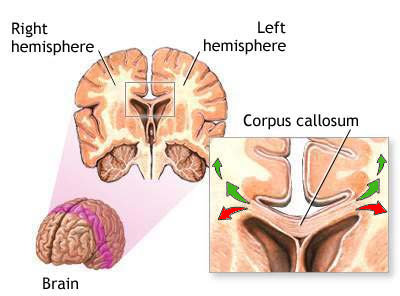
\includegraphics[width=0.5\linewidth]{figures/corpus_callosum_lateral.png} \\
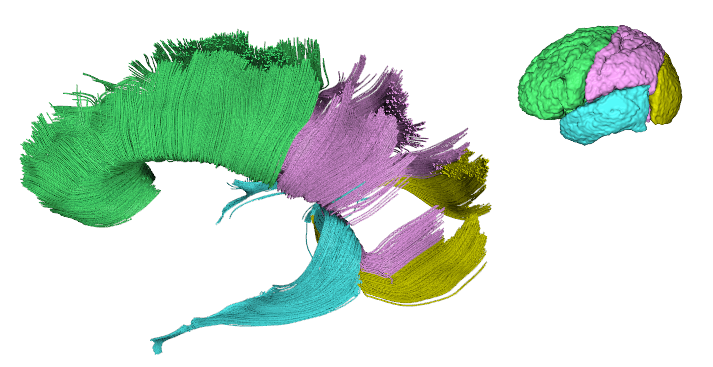
\includegraphics[width=0.8\linewidth]{figures/ccfibers2.png}
\caption{Above: The human corpus callosum (image adapted from~\cite{medlineplus}). Deterministic tractography methods are able to identify the aspects of the corpus callosum that connect superior cortical regions (green arrows), but are unable to identify the aspects that extend to more lateral cortical regions (red arrows). Below: Example results of atlas-based deterministic fiber tractography of the human corpus callosum with fibers colored by brain lobe. }
\label{fig:callosum}
\end{center}
\end{figure}

A centerline or skeletonization technique provides a method for avoiding bias caused by partial voluming that occurs in voxels that are not entirely within the white matter of the fiber tract of interest~\cite{Smith2006,Yushkevich2008}. Here we used a template-fiber approach. Each white matter tract was estimated as a set of streamlines, each of which was parametrized by arc-length to extend from 0.0 to 1.0. A BSpline was then fit to the set of all points from all streamlines in each bundle to obtain a single centerline that lies in the core of the fiber pathway of interest. For each point along the model pathway, a tangent was calculated and used to determine a perpendicular plane. The intersection of this plane with each of the streamlines in the bundle defined a set of points.  The normal and binormal vectors were used to re-parameterize the intersection points into 2D coordinates. Graham's scan method was used to determine the convex hull that encloses the set of intersection points~\cite{Graham1972}, and least-squared method was applied to the points on the hull to define an elliptical cross-section~\cite{Fitzgibbon1999}. To obtain a single FA value for the entire fiber bundle, the FA values were averaged over the length of the centerline.

\section{Results}

\subsection{Function}
The functional analyses revealed a network made up of 3 activated regions in the left hemisphere: dorsolateral prefrontal cortex (DLPFC), posterolateral temporal cortex (PLTC) and inferior frontal cortex (IFC). The region-averaged functional activation values are summarized in figure~\ref{fig:activations}. To identify activation changes that potentially result from aging, a Student's t-test was used to compare the young adults to all seniors for each ROI and suggested that activation in the right posterolateral cortex is greater in seniors (p=0.012). This same approach was used to identify potential differences between the cognitively matched and unmatched seniors. The cognitively matched seniors were found to have greater activation in the right dorsolateral prefrontal cortex (p=0.014) and reduced activation in the left posterolateral cortex (p=0.033) compared to the unmatched seniors.

\begin{figure}
\begin{center}
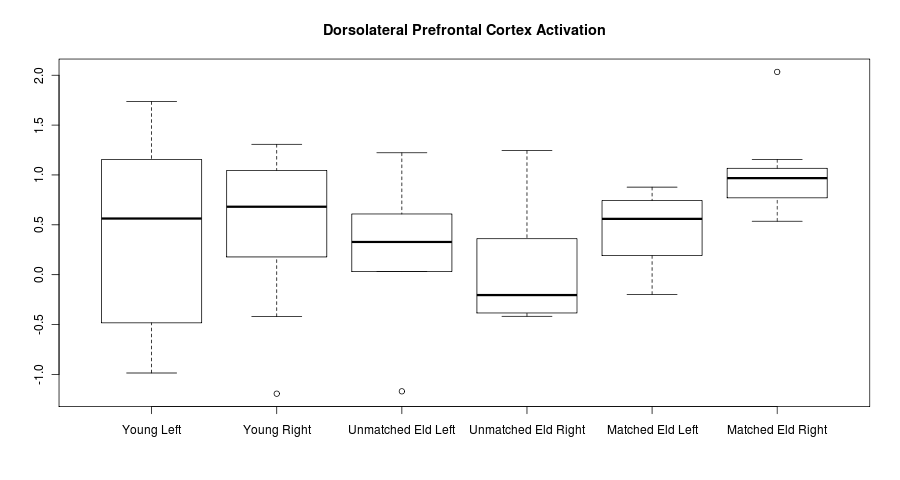
\includegraphics[width=0.8\linewidth]{figures/dlc_activation.png}\\
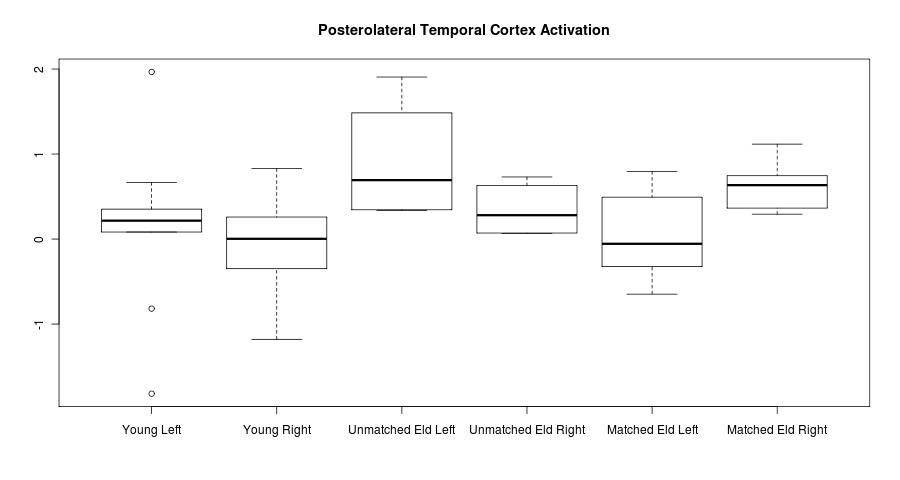
\includegraphics[width=0.8\linewidth]{figures/ptc_activation.png}\\
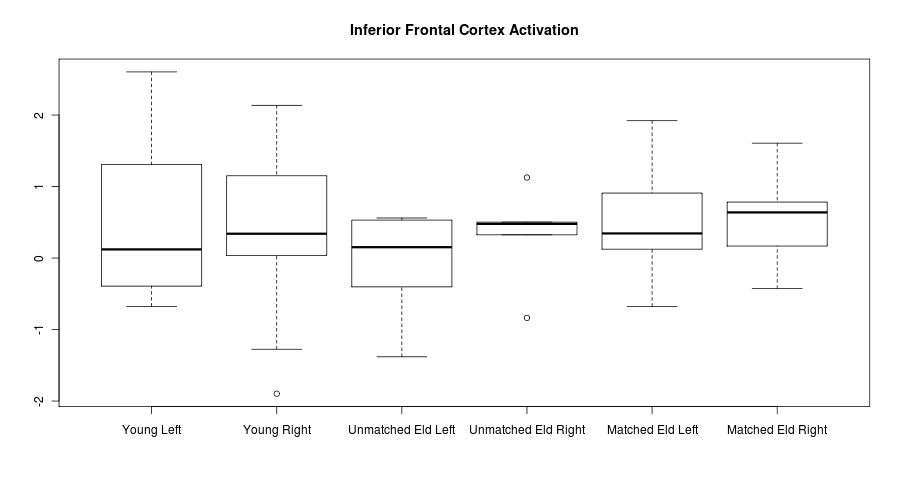
\includegraphics[width=0.8\linewidth]{figures/ifc_activation.png}
\caption{Region-averaged functional activation was measured in both hemispheres in the dorsolateral prefrontal cortex (top row), posterolateral temporal cortex (middle row) and inferior frontal cortex (bottom row).}
\label{fig:activations}
\end{center}
\end{figure}

\subsection{Structure}
The DTI tractography identified a network of connections made up of the arcuate fasciculus (right and left hemispheres), a bundle of short frontal fibers (right and left hemispheres), and 3 subcomponents of the corpus callosum. These fiber bundles were used to generate geometric models, illustrated in figure~\ref{fig:fibers}. A Student's t-test was used to identify potential differences between the young adults in seniors. Reduced FA in seniors compared to young adults was found in the inter-hemispheric connection between the PLTC regions (p=0.02889) and in the right short frontal fibers (p=0.00955). Increased FA in seniors was found in the right arcuate fasciculus (p=0.00747). Compared to lower performing seniors, higher performing seniors had lower FA in the inter-hemispheric connections between right and left IFC. 

\begin{figure}
\begin{center}
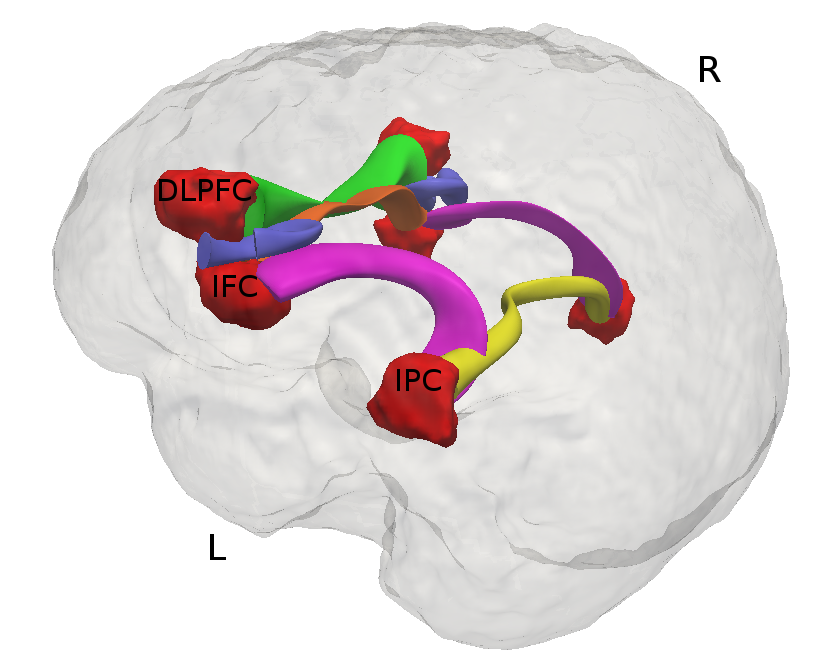
\includegraphics[width=0.9\linewidth]{figures/big_lat_labeled.png}
\caption{A set of 3 functionally activated regions: Dorsolateral Prefrontal Cortex (DLPFC), Posterolateral Temporal Cortex (PLTC), and Inferior Frontal Cortex (IFC) were identified in the left hemisphere. These regions, along with their right hemisphere homologues were used to identify the fiber tracts that provide biological connectivity. In each hemisphere, intra-hemispheric connectivity is provided by the arcuate fasciculus (pink) and a bundle of short frontal fibers (blue). Each homologous pair of activated regions was used to identify the following subcomponents of the corpus callosum that provided inter-hemispheric connectivity: DLPFC (green), IFC (orange) and PLTC (yellow). Surface-meshes created from the the geometric models are used for visualization of the white matter tracts.}
\label{fig:fibers}
\end{center}
\end{figure}

\begin{figure}
\begin{center}
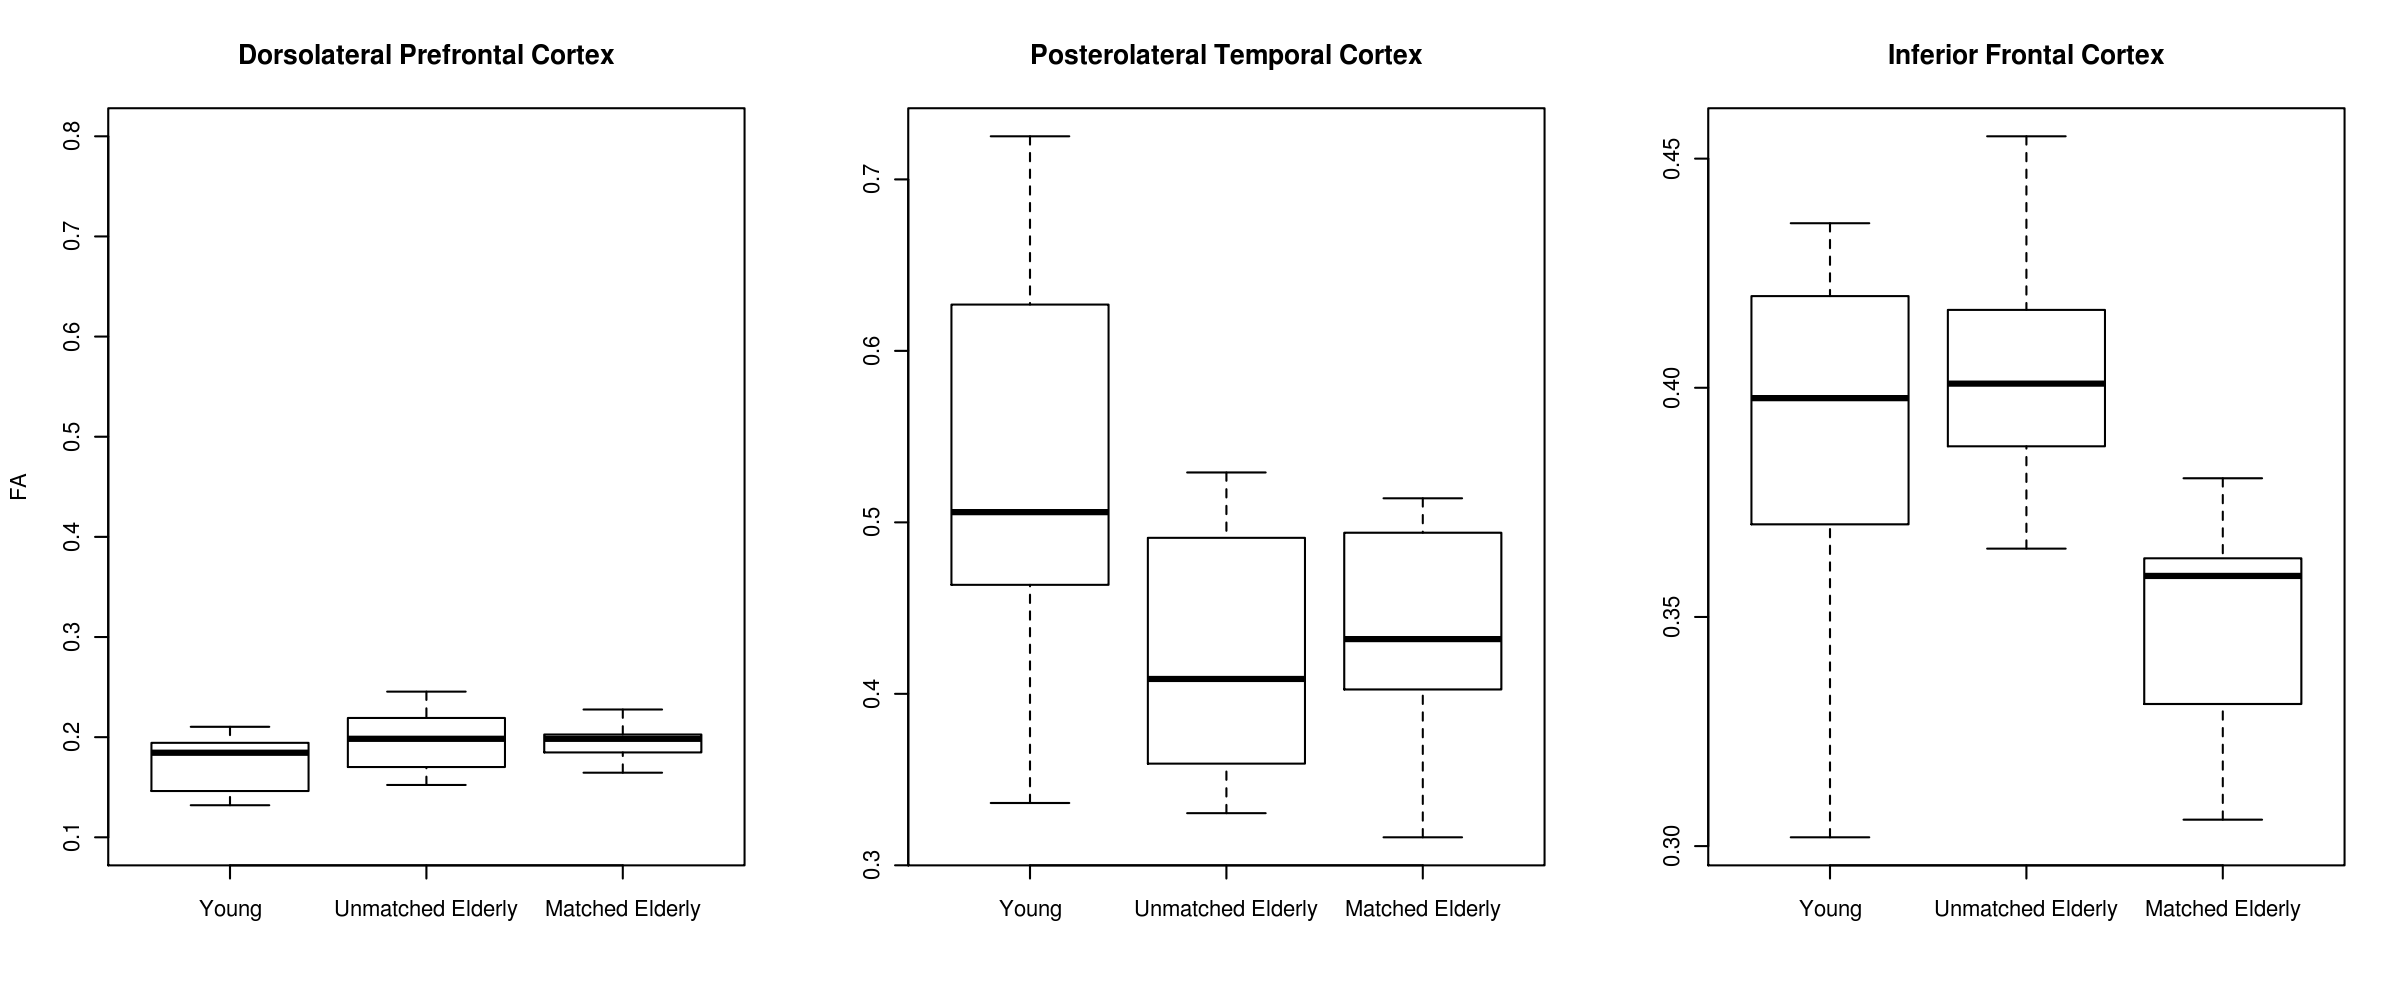
\includegraphics[width=1.0\linewidth]{figures/commissural.png}\\
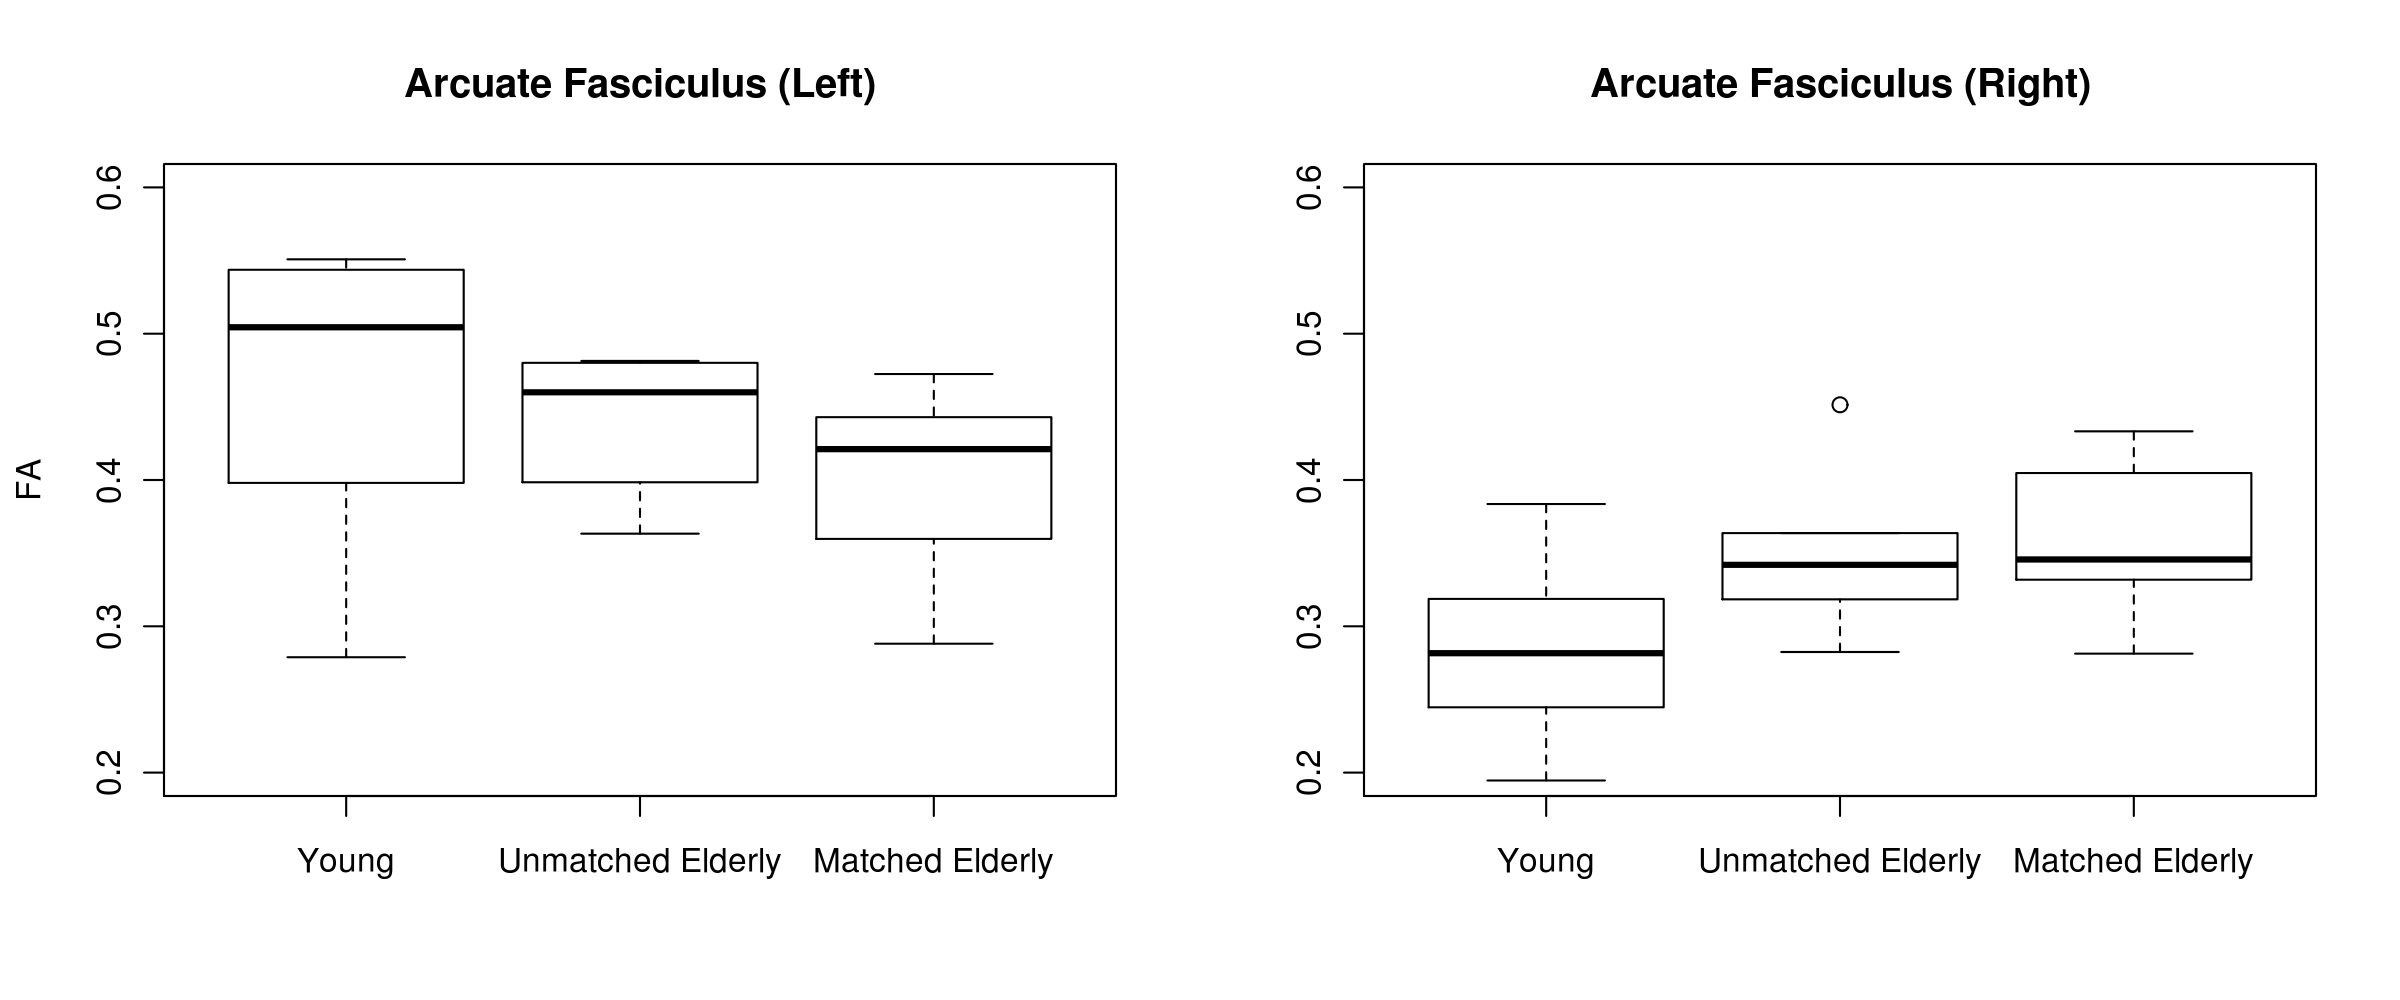
\includegraphics[width=0.8\linewidth]{figures/arcuate.png}\\
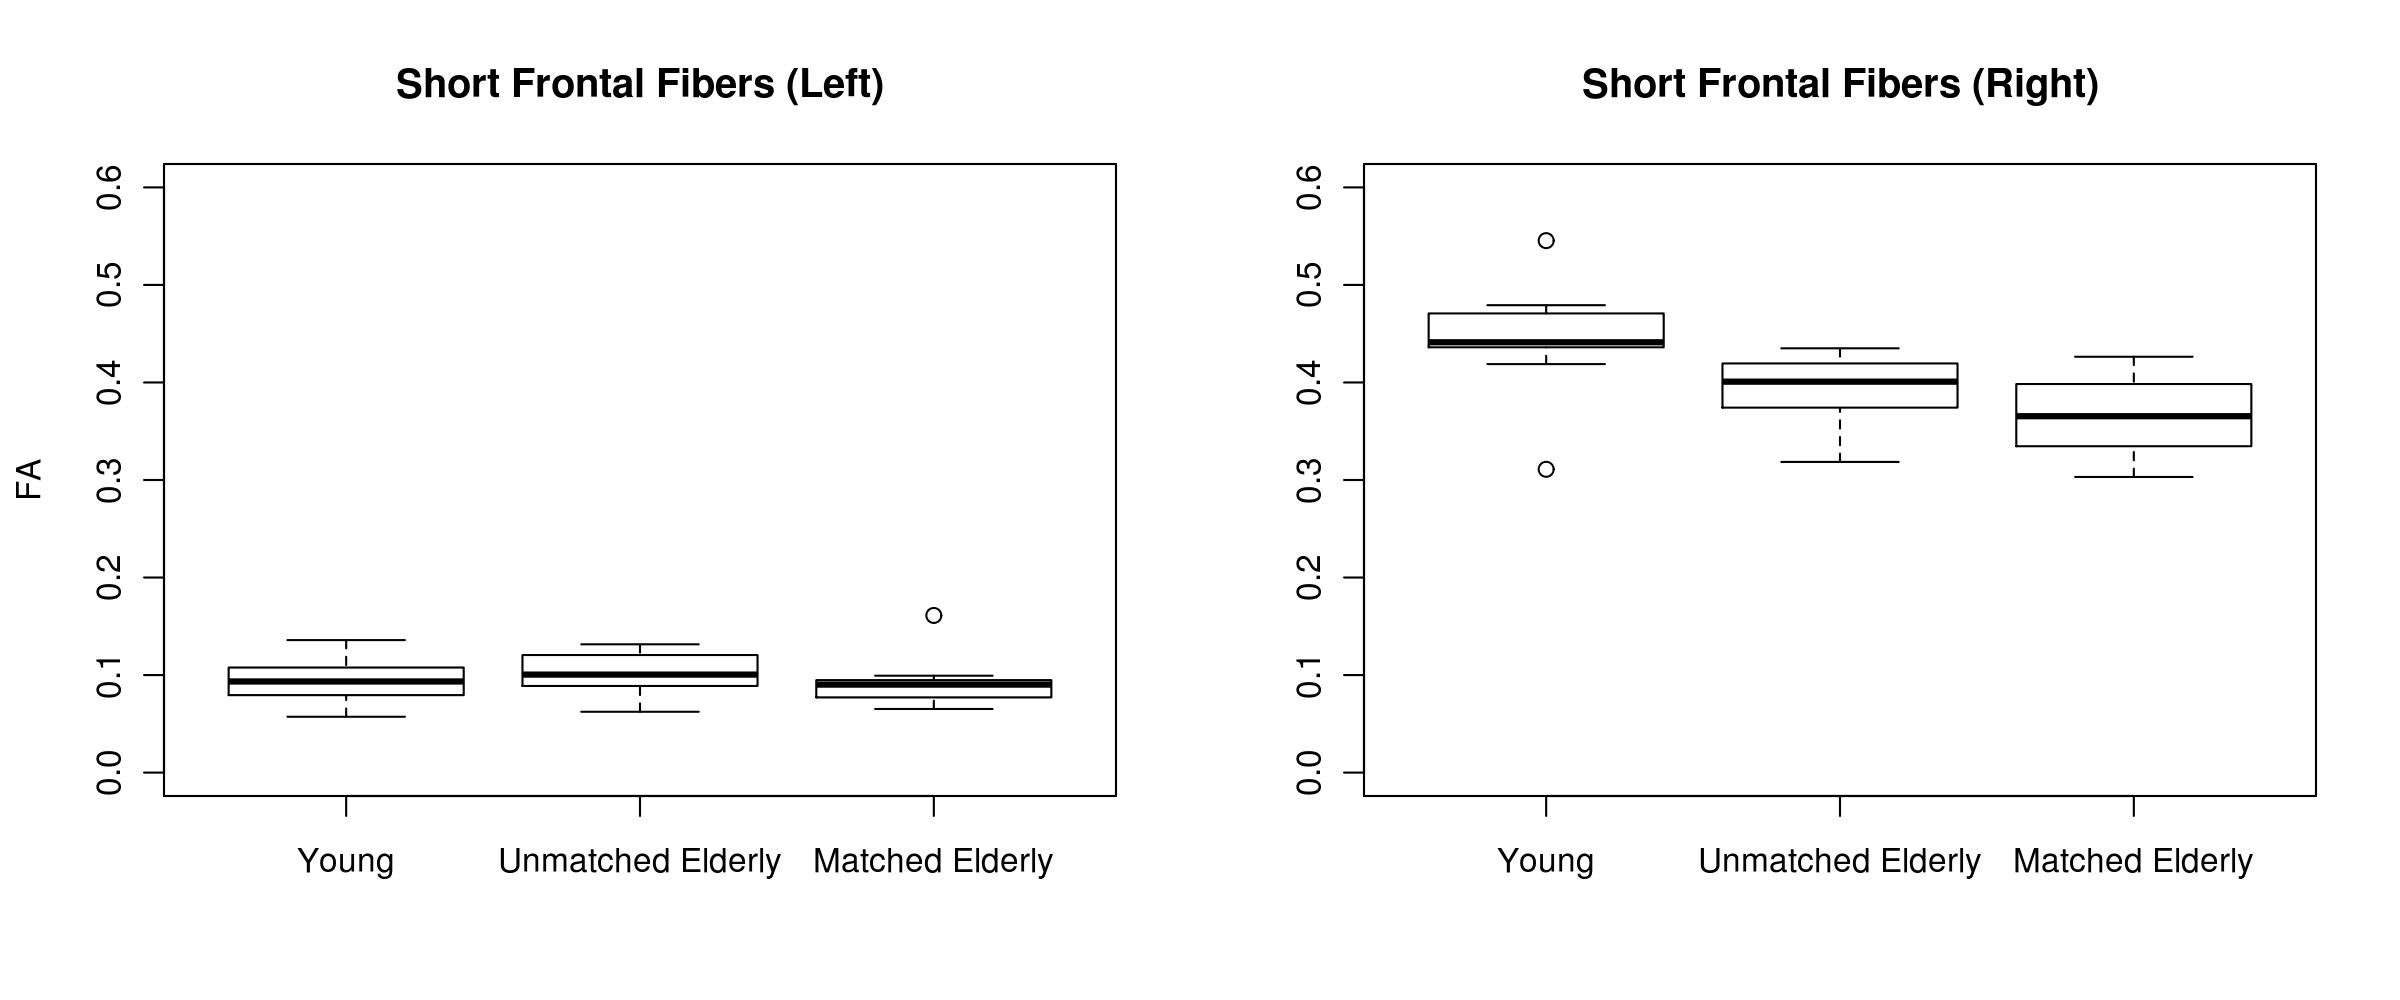
\includegraphics[width=0.8\linewidth]{figures/short.png}
\caption{Tract-averaged fractional anisotropy was measured for the portions of the corpus callosum that provide inter-hemispheric connections between the cortical regions of interest (top row), the arcuate fasciculus (middle row) and short frontal fibers (bottom row). }
\label{fig:fa}
\end{center}
\end{figure}

\section{Discussion}
This study demonstrated the potential for using combined analysis of fMRI and DTI in examining age-related changes in function and structure in the brain and how these changes regulate behavior. While language processing is primarily handled in the left hemisphere, the activation in young adults was symmetric. This is possibly a result of younger adults having an easier time processing the grammatically complex sentences due to intact neural resources. The finding of increased activation in the right PLTC of seniors is consistent with the \emph{compensation view} that right hemisphere brain function during language processing increases with age~\cite{Cabeza2002}. Also supporting this view is the finding of higher activation in the right DLPFC of higher performing (matched) seniors relative to lower performing (unmatched) seniors. The finding of increased left PLTC activation in lower performing seniors is also interesting in the context of activation patterns. Examining figure~\ref{fig:activations} reveals that lower performing seniors have a similar activation pattern to that of young adults (higher in left than right) with higher overall activation values. Higher performing seniors however have a different activation pattern (higher in right than left) suggesting that recruitment of right hemisphere resources is a more effective strategy for compensating for the effects of aging than maintaining a similar pattern to the young adult brain and increasing activation, supporting the \emph{psychogenic view}. While these results are interesting, the small number of subjects limited the scope of the study, and many of the findings would not stand-up to a family-wide (FWE) error correction. 

The finding of increased FA in the right hemispheric arcuate fasciculus and deceased FA in the short frontal fibers in the right hemisphere suggests that the increased functional recruitment of right hemispheric resources may be accompanied by white matter changes. The finding of reduced FA in the inter-hemispheric connections is also consistent with the \emph{compensation view} as these connections are thought to play an inhibitory role that aids in hemispheric specialization~\cite{Yazgan1995}. This is additionally supported by the finding of reduced FA in the PLTC connections of higher performing seniors compared to lower performing seniors who have similar FA values to those in young adults. However, due to the complicated composition of the corpus callosum, caution must be taken when interpreting FA values as FA is sensitive to a variety of white matte properties including but not limited to: myelination, axon diameter and density, fiber tract curvature, and intra-voxel fiber crossings~\cite{Barkovich2000,Shimony1999,Virta1999}. All of these factors are relevant in the corpus callosum which contains two different types of fibers (i.e. small diameter and large diameter) that make up independent subcomponents that may vary in density and degree of myelination and connect to different functionally specialized cortical regions. While our examination attempted to focus on connections between association regions, the mixing of fibers that occurs as fiber approach the mid-sagittal cross-section could cause a partial voluming bias based upon myelination differences in sensory-motor fibers. As demonstrated by Pierpaoli et al.\ \cite{Pierpaoli2001}, a selective decrease in the FA of one fiber population may result in an increase in FA within an individual voxel, and vice versa. Because of these issues, more work must be done to gain a deeper understanding of the physical basis for the structural changes detected here.

The use of template fibers with elliptical cross-sections provided an effective geometric model for examining white matter fiber bundle properties, and a great deal of opportunity exists for the development of more biologically relevant measures of structure. Here, these models were purely template-based and used to examine FA in individual subjects. Using these template-based models as a basis for fitting subject-specific models from subject-space tractography could potentially provide a more sensitive measure of structural integrity and could provide a framework that explicitly examines the geometry of white matter pathways as well as the properties of the underlying tissue. Additionally, the use of metrics that leverage the expected fiber orientation provided by the geometric model may be useful as they incorporate more widespread information about the fiber tract as opposed to the purely local measure provide by FA~\cite{duda08miccai}.

In order to examine functional activation in each hemisphere and identity connective pathways of the corpus callosum, cortical ROI's of equal volume were used. This is potentially problematic as language related regions such as Broca's area have been demonstrated to be larger in the left hemisphere and additionally varies a great deal between individuals~\cite{Galaburda1995}. This could potentially be addressed by incorporating the use of a cortical atlas in which cortical areas, such as Brodmann's areas, have been labeled. The use of a shortest-path fiber tracking method is dependent upon the a priori assumption that the target and seed regions are directly connected by a white matter tract. The low FA values found for the commisural connection of the DLPFC may suggest that rather than a direct connection, these regions may communicate via indirect connections via a combination of association and commisural fibers. 

In summary, an atlas-based approach was used to examine age-related changes in functional and structural lateralization. Seniors were found to have higher activation in the right PLTC and this activation was greater for higher performing seniors than lower performing seniors. Age-related increases and decreases in association fiber were found with FA in the right hemisphere arcuate fasciculus being higher in seniors, but FA in the right hemisphere short frontal fibers being lower in seniors. Reduced FA was found in the the posterolateral temporal inter-hemispheric connections of all seniors. Differences were found between high and low performing seniors in the commisural connections of the IFC with low performing seniors having FA values similar to the young adults and high performing seniors having reduced FA. These results suggests that age-related changes in both functional and structural lateralization have effects on cognitive performance, but the limited sample size and complex nature of the structures requires further examination.








